\chapter{Elektrodekinetiek en elektroanalyse}\label{ch:b3:electrode-kinetics}

Een druppel bloed op een plastic strookje, vijf seconden, een getal: de
glucosemeter die miljoenen mensen meerdere keren per dag gebruiken, is een
elektrochemische cel, en wat hij meet is geen spanning maar een stroom.
Een \omterm{def:b3:complex-kinetics:enzyme}{enzym} oxideert de glucose, een opgelost ijzercomplex brengt de
elektronen naar een koolstofelektrode, en de stroom die vloeit wordt
bepaald door de snelheid waarmee dat complex naar de elektrode
diffundeert, en dus door zijn concentratie. Dit hoofdstuk legt uit waarom
elektronen snel of traag een grensvlak oversteken (de \omterm{thm:b3:electrode-kinetics:butler-volmer}{vergelijking van
Butler-Volmer}), hoe stoftransport de stroom beperkt, en hoe \omterm{def:b3:electrode-kinetics:cv}{cyclische
voltammetrie} en de andere elektroanalytische methoden stromen omzetten in
concentraties, snelheidsconstanten en mechanismen.

\begin{recall}
Het deel van jaar~1 definieerde de elektrodepotentiaal, de
standaardpotentiaal, de vergelijking van Nernst, referentie-elektroden en
halfcellen. Het deel van jaar~2 voerde stroom-potentiaalkrommen in met hun
anodische en kathodische stromen, werk- en tegenelektroden,
overpotentialen, snelle en trage systemen, de diffusielaag en de
grensstroom; activiteitscoëfficiënten en ionsterkte; ijklijnen, de
standaardadditiemethode en de detectiegrens.
\Cref{ch:b3:rate-theories} gaf de \omterm{def:b3:rate-theories:tst}{overgangstoestandstheorie}. Uit de
natuurkunde: de wetten van Fick voor diffusie, de vergelijking van
Poisson en condensatoren.
\end{recall}

\begin{omfigure}
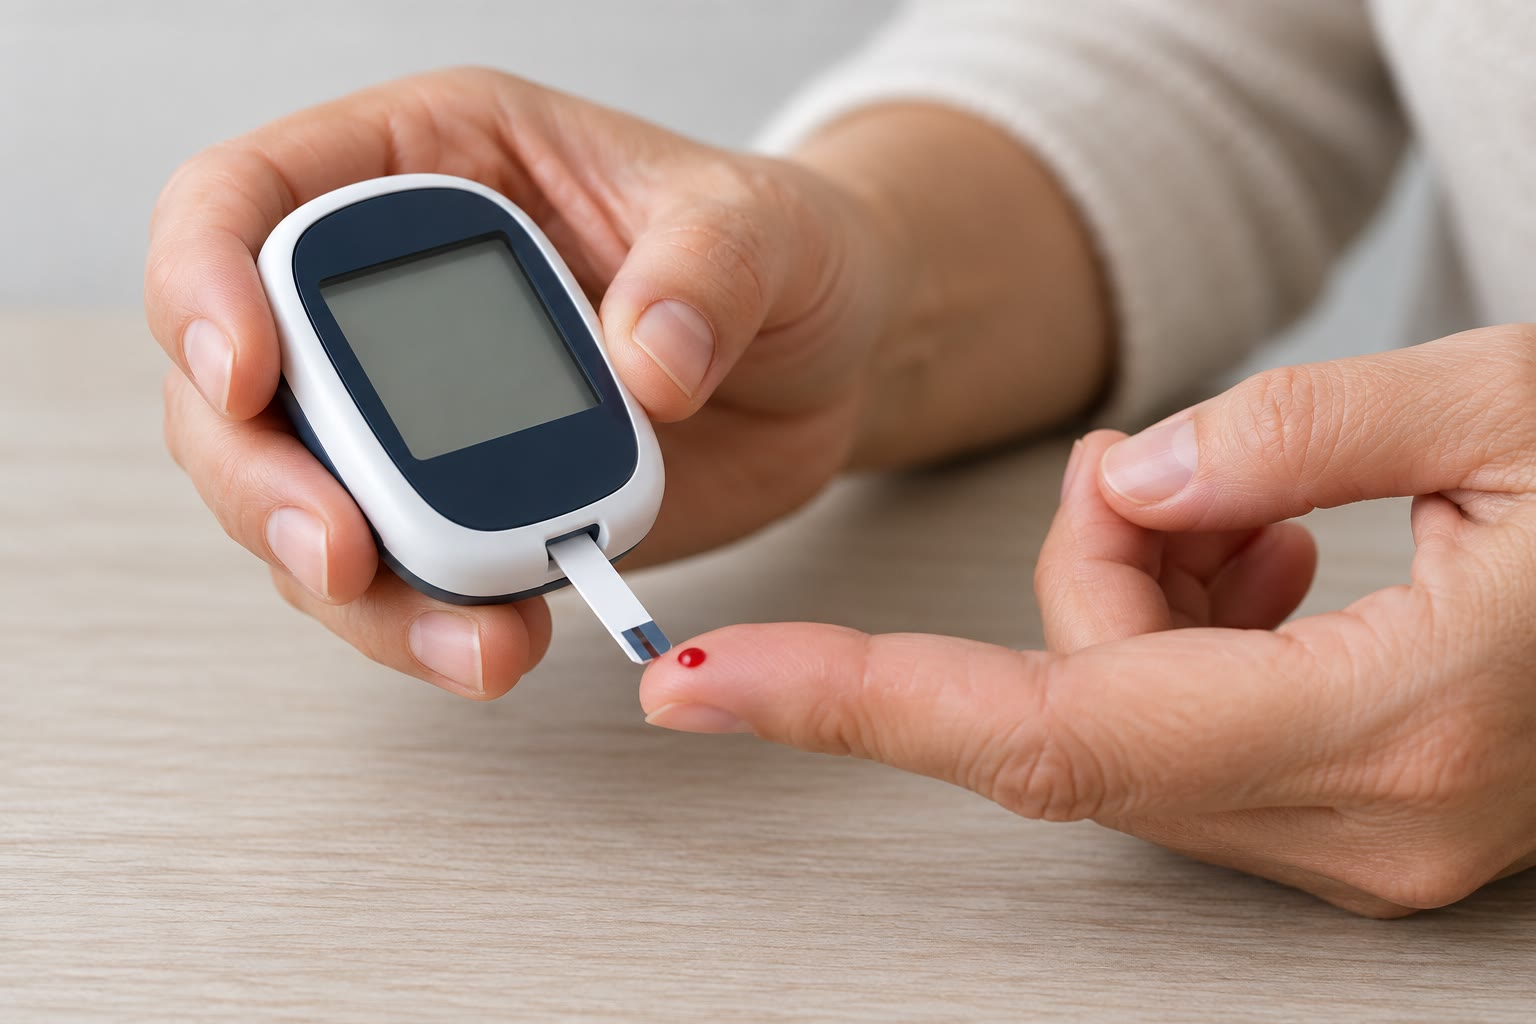
\includegraphics[width=0.6\linewidth]{images/book4/ai/b3-15-glucose-meter.jpg}

{\small Een bloedglucosemeter: het strookje draagt een minuscule cel met
drie elektroden, met een \omterm{def:b3:complex-kinetics:enzyme}{enzym} en een redoxmediator; de meter legt een
potentiaal aan en leest een stroom af.}
\end{omfigure}

\section{Het grensvlak elektrode-oplossing}

Een metaal dat in een elektrolytoplossing gedompeld wordt, draagt een
oppervlaktelading, en de oplossing antwoordt met een gelijke en
tegengestelde lading, gevormd door een overmaat ionen van één teken. De
twee ladingslagen vormen een condensator van moleculaire dikte.

\begin{definition}[Elektrische dubbellaag]\label{def:b3:electrode-kinetics:double-layer}
De \emph{elektrische dubbellaag}\index{elektrische dubbellaag} is de
schikking van lading aan een grensvlak elektrode-oplossing: de lading op
het metaal en de compenserende ionenlading in de oplossing. Haar compacte
deel, de
\emph{helmholtzlaag}\index{helmholtzlaag}, is de laag ionen en
oplosmiddelmoleculen die het oppervlak raakt; haar
\emph{diffuse laag}\index{diffuse laag}
is het gebied daarbuiten, waar de thermische beweging de overmaat ionen
spreidt over een afstand van de orde van de
\emph{debyelengte}\index{debyelengte} $\kappa^{-1}$. De
\emph{dubbellaagcapaciteit}\index{dubbellaagcapaciteit} $C_{\mathrm{dl}}$
is de lading die per oppervlakte-eenheid opgeslagen wordt per volt
potentiaal over het grensvlak.
\end{definition}

\begin{proposition}[Debyelengte]\label{prop:b3:electrode-kinetics:debye-length}
In een oplossing met ionsterkte $I$ (in \unit{mol.m^{-3}}) en relatieve
permittiviteit
$\varepsilon_r$ neemt een kleine potentiaal $\varphi_0$ aan de elektrode in
de oplossing af als
$\varphi = \varphi_0\eu^{-\kappa x}$, met
\[
  \kappa^{-1} = \sqrt{\frac{\varepsilon_r\varepsilon_0RT}{2F^2I}} .
\]
\end{proposition}

\begin{proof}
De vergelijking van Poisson (uit de natuurkunde) verbindt de potentiaal
met de ladingsdichtheid:
$\dd^2\varphi/\dd x^2 = -\rho/\varepsilon_r\varepsilon_0$. Elk ion volgt in de
potentiaal de \omterm{def:b3:partition-functions:boltzmann}{boltzmannverdeling}: $c_i = c_i^{\circ}\eu^{-z_iF\varphi/RT}$, zodat $\rho = F\sum_iz_ic_i^{\circ}\eu^{-z_iF\varphi/RT}$. Voor $F\varphi \ll RT$
is
$\eu^{-z_iF\varphi/RT} \approx 1 - z_iF\varphi/RT$; de termen van orde nul vallen weg door de
elektroneutraliteit,
en $\rho \approx -(F^2/RT)\sum_iz_i^2c_i^{\circ}\,\varphi = -(2F^2I/RT)\varphi$. Dus $\dd^2\varphi/\dd x^2 = \kappa^2\varphi$, met als
oplossing die ver weg nul wordt $\varphi_0\eu^{-\kappa x}$.
\end{proof}

\begin{example}[De dikte van de dubbellaag]\label{ex:b3:electrode-kinetics:debye}
% ledger: eps:H2O.25C, const:eps0, const:F, const:R
In water bij \qty{298.15}{K} ($\varepsilon_r = 78.4$) met
\qty{0.10}{mol/L} van een 1:1-zout ($I = \qty{100}{mol.m^{-3}}$) is
$\kappa^{-1} = \sqrt{78.4 \times \num{8.854e-12} \times 2479/(2 \times 96\,485^2 \times 100)} = \qty{0.96}{nm}$; bij \qty{1.0}{mmol/L}
tien keer meer. Een \omterm{def:b3:electrode-kinetics:transport}{leidzout} drukt de \omterm{def:b3:electrode-kinetics:double-layer}{diffuse laag} samen tot enkele
moleculaire diameters.
\end{example}

De \omterm{def:b3:electrode-kinetics:double-layer}{diffuse laag} gedraagt zich als een condensator waarvan de platen
$\kappa^{-1}$ uit elkaar liggen: haar capaciteit per oppervlakte-eenheid
bij lage potentiaal is $\varepsilon_r\varepsilon_0\kappa$ (het resultaat
van Gouy-Chapman; de afhankelijkheid van de potentiaal wordt aangenomen).
In serie met de compacte \omterm{def:b3:electrode-kinetics:double-layer}{helmholtzlaag} geeft ze de gemeten $C_{\mathrm{dl}}$, van de orde van tientallen
microfarad per vierkante centimeter (het model van Stern). Telkens wanneer
de potentiaal verandert, laadt deze condensator op: een scan met $v$ volt
per seconde trekt een laadstroom $C_{\mathrm{dl}}Av$ die geen chemie
draagt en bij elke voltammetrische meting opgeteld wordt.

\begin{omfigure}
\begin{tikzpicture}[font=\small, >=Stealth]
  \fill[black!25] (-1.0,0) rectangle (0,3.2);
  \node[rotate=90] at (-0.5,1.6) {metaal};
  \foreach \y in {0.3,0.8,...,2.9}{\node[font=\scriptsize] at (-0.15,\y) {$-$};}
  \foreach \y in {0.35,0.95,1.55,2.15,2.75}{\draw[omDef, fill=omDef!20] (0.3,\y) circle (0.18); \node[font=\scriptsize] at (0.3,\y) {$+$};}
  \draw[black!50, dashed] (0.55,0) -- (0.55,3.2);
  \node[font=\scriptsize, anchor=south, align=center] at (0.45,3.25) {helmholtz-\\ vlak};
  \foreach \x/\y/\s in {1.1/0.6/+, 1.4/2.2/+, 1.9/1.3/+, 2.3/2.7/-, 2.6/0.5/+, 3.1/1.8/+, 3.5/0.9/-, 3.9/2.4/+, 4.4/1.4/-, 4.8/0.4/+, 5.1/2.8/-, 5.4/1.9/+}{
    \draw[black!60, fill=white] (\x,\y) circle (0.15); \node[font=\scriptsize] at (\x,\y) {$\s$};}
  \node[font=\scriptsize, anchor=south] at (3.2,3.25) {diffuse laag};
  \draw[->] (0,-2.1) -- (6.0,-2.1) node[anchor=north east] {$x$};
  \draw[->] (0,-2.1) -- (0,-0.3) node[anchor=east] {$|\varphi|$};
  \draw[omThm, thick] (0,-0.5) -- (0.55,-1.0) plot[domain=0.55:5.8, samples=40] (\x,{-2.1+1.1*exp(-(\x-0.55)/1.2)});
  \draw[black!40, dashed] (0.55,-2.1) -- (0.55,-0.4);
  \node[omThm, anchor=south west] at (1.3,-1.6) {$|\varphi(x)|$};
  \draw[<->, black!60] (0.55,-2.5) -- (1.75,-2.5) node[midway, below, font=\scriptsize] {$\sim\kappa^{-1}$};
\end{tikzpicture}

{\small De \omterm{def:b3:electrode-kinetics:double-layer}{elektrische dubbellaag} (model van Gouy-Chapman-Stern,
schematisch): een negatief geladen metaal, een compacte laag kationen in
het helmholtzvlak, en een \omterm{def:b3:electrode-kinetics:double-layer}{diffuse laag} waarin kationen over enkele
\omterm{def:b3:electrode-kinetics:double-layer}{debyelengten} in de meerderheid zijn. Onder: de grootte van de potentiaal
(negatief, zoals de lading van het metaal) daalt lineair over de compacte
laag, daarna exponentieel in de \omterm{def:b3:electrode-kinetics:double-layer}{diffuse laag}.}
\end{omfigure}

\section{Kinetiek van elektronenoverdracht}

Beschouw de reductie $\mathrm{O} + n\,\mathrm{e}^- \to \mathrm{R}$ aan een
elektrode die op de potentiaal $E$ gehouden wordt, waarvan de
evenwichtspotentiaal voor de bulkoplossing $E_{\mathrm{eq}}$ zou zijn. De
overpotentiaal is $\eta = E - E_{\mathrm{eq}}$.

\begin{definition}[Uitwisselingsstroomdichtheid, overdrachtscoëfficiënt, standaardsnelheidsconstante]\label{def:b3:electrode-kinetics:exchange}
In evenwicht zijn de anodische en de kathodische stroom gelijk en
tegengesteld; hun gemeenschappelijke grootte per oppervlakte-eenheid is de
\emph{uitwisselingsstroomdichtheid}\index{uitwisselingsstroomdichtheid}
$j_0$. De \emph{overdrachtscoëfficiënt}
\index{overdrachtscoefficient@overdrachtscoëfficiënt} $\alpha$ ($0 < \alpha < 1$) is de fractie van de
elektrische energie $nF\eta$ die de barrière van de kathodische reactie
verlaagt. De
\emph{standaardsnelheidsconstante}\index{standaardsnelheidsconstante}
$k^\circ$ is de gemeenschappelijke waarde van de kathodische en de
anodische snelheidsconstante bij de formele potentiaal $E^{\circ\prime}$.
\end{definition}

\begin{theorem}[Vergelijking van Butler-Volmer]\label{thm:b3:electrode-kinetics:butler-volmer}
Als de oppervlakteconcentraties gelijk zijn aan die in de bulk (geen
beperking door stoftransport), is de stroomdichtheid bij overpotentiaal
$\eta$, met anodische stromen positief geteld,
\[
  j = j_0\bigl[\eu^{(1 - \alpha)f\eta} - \eu^{-\alpha f\eta}\bigr], \qquad f = \frac{nF}{RT}.
\]
Dit is de \emph{vergelijking van Butler-Volmer}\index{vergelijking van Butler-Volmer}.
\end{theorem}

\begin{proof}
Volgens de \omterm{def:b3:rate-theories:tst}{overgangstoestandstheorie} zijn de kathodische en de anodische
snelheidsconstante
$k_{\mathrm c} = A\eu^{-\Delta G_{\mathrm c}^{\ddagger}/RT}$ en $k_{\mathrm a} = A\eu^{-\Delta G_{\mathrm a}^{\ddagger}/RT}$. Een verandering van de elektrodepotentiaal met $\delta E$
verandert de gibbsenergie van de reactie $\mathrm{O} + n\,\mathrm{e}^- \to \mathrm{R}$ met $nF\,\delta E$ (de elektronen
in het metaal winnen $-nF\,\delta E$ aan elektrische energie). Neem in
eerste orde aan dat een fractie $\alpha$ van deze verandering in de
kathodische barrière terechtkomt en de rest in de anodische: $\Delta G_{\mathrm c}^{\ddagger} \to \Delta G_{\mathrm c}^{\ddagger} + \alpha nF\,\delta E$, $\Delta G_{\mathrm a}^{\ddagger} \to \Delta G_{\mathrm a}^{\ddagger} - (1 - \alpha)nF\,\delta E$. Meten van $\delta E$
vanaf de evenwichtspotentiaal, waar beide stromen in grootte $j_0$ zijn,
geeft $j_{\mathrm c} = j_0\eu^{-\alpha f\eta}$ en $j_{\mathrm a} = j_0\eu^{(1 - \alpha)f\eta}$; de nettostroom is hun
verschil.
\end{proof}

\begin{corollary}[Ladingsoverdrachtsweerstand]\label{cor:b3:electrode-kinetics:linear}
Voor $|\eta| \ll RT/nF$ is $j = j_0f\eta$: het grensvlak gedraagt zich als
een weerstand
$R_{\mathrm{ct}} = RT/(nFi_0)$, met $i_0 = j_0A$.
\end{corollary}

\begin{proof}
Ontwikkel beide exponentiëlen tot de eerste orde: $j = j_0[(1 - \alpha)f\eta + \alpha f\eta] = j_0f\eta$; dan is
$\eta/i = 1/(fi_0)$.
\end{proof}

\begin{corollary}[Vergelijking van Tafel]\label{cor:b3:electrode-kinetics:tafel}
Voor $\eta \ll -RT/nF$ (een sterk kathodische overpotentiaal) is de
anodische term verwaarloosbaar en
\[
  \eta = \frac{2.303\,RT}{\alpha nF}\bigl(\log j_0 - \log|j|\bigr):
\]
$\log|j|$ is lineair in $\eta$, met een helling van $1/(\text{\qty{118}{mV}})$ per decade bij \qty{298}{K} voor $\alpha = 0.5$, $n =
1$. Dit is de \emph{vergelijking van Tafel}\index{vergelijking van Tafel}.
\end{corollary}

\begin{proof}
$|j| = j_0\eu^{-\alpha f\eta}$, dus $\ln|j| = \ln j_0 - \alpha f\eta$; zet om naar
decimale logaritmen.
\end{proof}

\begin{definition}[Ladingsoverdrachtsweerstand, tafelhelling]\label{def:b3:electrode-kinetics:charge-transfer}
De \emph{ladingsoverdrachtsweerstand}\index{ladingsoverdrachtsweerstand}
van een elektrode is $R_{\mathrm{ct}} = (\partial\eta/\partial i)_{\eta = 0}$. De
\emph{tafelhelling}\index{tafelhelling}
is de verandering van de overpotentiaal per decade stroom in het
tafelgebied,
$2.303\,RT/\alpha nF$.
\end{definition}

\begin{omfigure}
\begin{tikzpicture}
\begin{axis}[name=bv, omcv, width=0.47\linewidth, height=5.4cm, xmin=-300, xmax=300, ymin=-40, ymax=40,
  xlabel={$\eta$ / mV}, ylabel={$j/j_0$},
  legend style={font=\scriptsize, draw=none, at={(0.03,0.97)}, anchor=north west}, legend cell align=left]
\addplot[omDef, thick] table[x=eta_mV, y=a3] {figdata/out/bachelor-3-butler-volmer.dat};
\addplot[black, thick] table[x=eta_mV, y=a5] {figdata/out/bachelor-3-butler-volmer.dat};
\addplot[omThm, thick] table[x=eta_mV, y=a7] {figdata/out/bachelor-3-butler-volmer.dat};
\legend{$\alpha = 0.3$, $\alpha = 0.5$, $\alpha = 0.7$}
\draw[black!30] (axis cs:-300,0) -- (axis cs:300,0) (axis cs:0,-40) -- (axis cs:0,40);
\end{axis}
\begin{axis}[at={(bv.east)}, anchor=west, xshift=1.2cm, omcv, width=0.47\linewidth, height=5.4cm,
  xmin=-300, xmax=300, ymin=-1.5, ymax=4, xlabel={$\eta$ / mV}, ylabel={$\log|j/j_0|$},
  unbounded coords=jump]
\addplot[omDef, thick] table[x=eta_mV, y=l3] {figdata/out/bachelor-3-butler-volmer.dat};
\addplot[black, thick] table[x=eta_mV, y=l5] {figdata/out/bachelor-3-butler-volmer.dat};
\addplot[omThm, thick] table[x=eta_mV, y=l7] {figdata/out/bachelor-3-butler-volmer.dat};
\draw[black!40, dashed] (axis cs:-300,2.54) -- (axis cs:0,0);
\draw[black!50] (axis cs:-200,1.85) -- (axis cs:-120,3.3) node[anchor=south, font=\scriptsize, inner sep=1pt] {helling $1/(\qty{118}{mV})$};
\end{axis}
\end{tikzpicture}

{\small De \omterm{thm:b3:electrode-kinetics:butler-volmer}{vergelijking van Butler-Volmer} ($n = 1$, \qty{298}{K}) voor drie
\omterm{def:b3:electrode-kinetics:exchange}{overdrachtscoëfficiënten}. Links: de stroom is lineair in $\eta$ nabij het
evenwicht (de \omterm{def:b3:electrode-kinetics:charge-transfer}{ladingsoverdrachtsweerstand}) en exponentieel daarbuiten;
$\alpha$ maakt hem asymmetrisch.
Rechts: de tafelgrafiek, waarvan de rechte takken extrapoleren naar
$\log|j/j_0| = 0$ bij $\eta = 0$; de gestreepte lijn is de kathodische
tafelrechte voor $\alpha = 0.5$.}
\end{omfigure}

\begin{method}[Een tafelanalyse]\label{met:b3:electrode-kinetics:tafel-analysis}
\begin{enumerate}
  \item Meet de stationaire stroom als functie van $\eta$ in een geroerde
        oplossing, ruim onder de grensstroom (of corrigeer voor het
        stoftransport).
  \item Zet $\log|i|$ uit tegen $\eta$; pas de lineaire tak voorbij
        ongeveer \qty{100}{mV} aan.
  \item De helling geeft $\alpha$ (of $1 - \alpha$ op de anodische tak); de
        afsnijding bij $\eta = 0$ geeft $\log i_0$.
  \item Controle: nabij $\eta = 0$ is de helling van $i$ tegen $\eta$ gelijk
        aan $1/R_{\mathrm{ct}} = nFi_0/RT$.
\end{enumerate}
\end{method}

De snelle en trage systemen uit het deel van jaar~2 zijn de twee
uitersten van dit beeld: een snel systeem heeft een grote $j_0$ en zijn
stroom-potentiaalkromme stijgt steil bij de evenwichtspotentiaal; een
traag systeem heeft een grote overpotentiaal nodig voordat er stroom
vloeit. De \omterm{def:b3:electrode-kinetics:exchange}{uitwisselingsstroomdichtheid} van dezelfde reactie varieert over
vele grootteordes van het ene elektrodemateriaal tot het andere: de
waterstofontwikkeling is snel op platina en uiterst traag op kwik.

\section{Stoftransport}

\begin{definition}[Vormen van stoftransport]\label{def:b3:electrode-kinetics:transport}
Deeltjes bereiken een elektrode door \emph{migratie}\index{migratie}, de
beweging van ionen in het elektrisch veld; door diffusie, langs
concentratiegradiënten; en door \emph{convectie}\index{convectie}, de
beweging van de oplossing als geheel (roeren, rotatie, stroming). Een
\emph{leidzout}\index{leidzout}
is een inert zout dat in grote overmaat toegevoegd wordt en bijna alle
stroom door de oplossing voert, zodat het elektroactieve deeltje alleen
door diffusie en convectie beweegt.
\end{definition}

\begin{definition}[Chronoamperometrie]\label{def:b3:electrode-kinetics:chronoamperometry}
\emph{Chronoamperometrie}\index{chronoamperometrie} registreert de stroom
als functie van de tijd na een sprong van de elektrodepotentiaal.
\end{definition}

\begin{theorem}[Vergelijking van Cottrell]\label{thm:b3:electrode-kinetics:cottrell}
Na een potentiaalsprong op $t = 0$ naar een waarde waarbij het
elektroactieve deeltje verbruikt wordt zodra het een vlakke elektrode met
oppervlakte $A$ bereikt, in een rustige oplossing met een \omterm{def:b3:electrode-kinetics:transport}{leidzout}, is
de stroom
\[
  i = nFAc^*\sqrt{\frac{D}{\pi t}},
\]
waarin $c^*$ de bulkconcentratie is en $D$ de diffusiecoëfficiënt. Dit is
de \emph{vergelijking van Cottrell}\index{vergelijking van Cottrell}.
\end{theorem}

\begin{proof}
De concentratie gehoorzaamt aan de tweede wet van Fick $\partial c/\partial t = D\,\partial^2c/\partial x^2$, met $c(x, 0) = c^*$,
$c(0, t) = 0$ voor $t > 0$ en $c \to c^*$ ver weg. De functie $c = c^*\operatorname{erf}(x/2\sqrt{Dt})$, met
$\operatorname{erf}u = \frac{2}{\sqrt\pi}\int_0^u\eu^{-s^2}\dd s$, voldoet aan deze voorwaarden: $\operatorname{erf}0 = 0$, $\operatorname{erf}u \to 1$ als $u \to \infty$
(bij $t \to 0$ voor elke $x > 0$, en ver weg). Met $u = x/2\sqrt{Dt}$ is
$\partial c/\partial t = c^*\frac{2}{\sqrt\pi}\eu^{-u^2}\partial u/\partial t = -c^*\frac{2}{\sqrt\pi}\eu^{-u^2}\frac{u}{2t}$ en $\partial^2c/\partial x^2 = c^*\frac{2}{\sqrt\pi}(-2u)\eu^{-u^2}\frac{1}{4Dt}$: de
twee leden van de wet van Fick stemmen overeen. De stroom is de flux aan het oppervlak: $i =
nFAD(\partial c/\partial x)_{x = 0} = nFADc^*\frac{2}{\sqrt\pi}\frac{1}{2\sqrt{Dt}} = nFAc^*\sqrt{D/\pi t}$. (De
uniciteit van de oplossing wordt aangenomen.)
\end{proof}

\begin{omfigure}
\begin{tikzpicture}
\begin{axis}[name=pr, width=0.47\linewidth, height=5.2cm, xmin=0, xmax=600, ymin=0, ymax=1.08,
  axis lines=left, xlabel={$x$ / \unit{\micro m}}, ylabel={$c/c^*$},
  tick label style={font=\small}, label style={font=\small},
  legend style={font=\scriptsize, draw=none, at={(0.97,0.03)}, anchor=south east}, legend cell align=left]
\addplot[omDef, thick] table[x=x_um, y=t1] {figdata/out/bachelor-3-cottrell-profiles.dat};
\addplot[black!60, thick] table[x=x_um, y=t2] {figdata/out/bachelor-3-cottrell-profiles.dat};
\addplot[omThm, thick] table[x=x_um, y=t3] {figdata/out/bachelor-3-cottrell-profiles.dat};
\addplot[black, thick, dashed] table[x=x_um, y=t4] {figdata/out/bachelor-3-cottrell-profiles.dat};
\legend{\qty{0.1}{s}, \qty{1}{s}, \qty{4}{s}, \qty{16}{s}}
\end{axis}
\begin{axis}[at={(pr.east)}, anchor=west, xshift=1.3cm, width=0.47\linewidth, height=5.2cm,
  xmin=0, xmax=3.3, ymin=0, ymax=40, axis lines=left, xlabel={$t^{-1/2}$ / \unit{s^{-1/2}}},
  ylabel={$i$ / \unit{\micro A}}, tick label style={font=\small}, label style={font=\small}]
\addplot[omDef, very thick] table[x=tm12, y=i_uA] {figdata/out/bachelor-3-cottrell-current.dat};
\end{axis}
\end{tikzpicture}

{\small \omterm{def:b3:electrode-kinetics:chronoamperometry}{Chronoamperometrie} (model: $D = \qty{1.0e-5}{cm^2.s^{-1}}$, $c^* = \qty{1.0}{mM}$, een
schijfje van \qty{3}{mm}). Links: de verarmde laag groeit als $\sqrt{Dt}$,
ongeveer \qty{30}{\micro m} na \qty{0.1}{s}
en \qty{350}{\micro m} na \qty{16}{s}. Rechts: de stroom van Cottrell is
evenredig met
$t^{-1/2}$; zijn helling geeft $D$.}
\end{omfigure}

Een geroerde oplossing of een roterende schijfelektrode houdt de
diffusielaag op een constante dikte $\delta$: de stroom bereikt de
stationaire grenswaarde $nFADc^*/\delta$ uit het deel van jaar~2. Voor een
roterende schijf neemt $\delta$ af als de inverse vierkantswortel van de
rotatiesnelheid (Levich, aangenomen), wat de grensstroom evenredig maakt
met $\sqrt\omega$.

\section{Cyclische voltammetrie}

\begin{definition}[Cyclische voltammetrie]\label{def:b3:electrode-kinetics:cv}
\emph{Cyclische voltammetrie}\index{cyclische voltammetrie} laat de
potentiaal van een stilstaande werkelektrode lineair met de tijd heen en
terug lopen tussen twee grenzen, met een scansnelheid $v$, in een rustige
oplossing, en registreert de stroom. De grafiek van de stroom tegen de
potentiaal is het \emph{voltammogram}\index{voltammogram}; elke golf heeft
een \emph{piekstroom}\index{piekstroom} $i_{\mathrm p}$ bij haar
\emph{piekpotentiaal}\index{piekpotentiaal}
$E_{\mathrm p}$.
\end{definition}

De piek ontstaat uit twee concurrerende effecten. Naarmate de potentiaal
voorbij $E^{\circ\prime}$ gaat, daalt de oppervlakteconcentratie van de
beginstof (de vergelijking van Nernst, voor een snel systeem) en groeit
de stroom; maar de verarmde laag wordt dikker met de tijd en de flux
daalt. Bij de terugscan wordt het product, dat nog dicht bij de
elektrode is, teruggezet.

\begin{definition}[Reversibiliteit]\label{def:b3:electrode-kinetics:reversibility}
Met de dimensieloze snelheidsparameter $\Lambda = k^\circ/\sqrt{DnFv/RT}$,
die de snelheid van de elektronenoverdracht vergelijkt met de snelheid
van diffusie die de scan oplegt, is een koppel
\emph{elektrochemisch reversibel}\index{elektrochemisch reversibel systeem}
als $\Lambda > 15$ (zijn oppervlakteconcentraties volgen op elk ogenblik de
vergelijking van Nernst),
\emph{quasi-reversibel}\index{quasi-reversibel systeem} als $15 >
\Lambda > 10^{-2(1 + \alpha)}$, en
\emph{elektrochemisch irreversibel}\index{elektrochemisch irreversibel systeem}
daaronder.
\end{definition}

\begin{remark}
De snelle en trage systemen uit het deel van jaar~2 komen overeen met deze
indeling, maar met een verschil: de reversibiliteit hangt hier af van de
scansnelheid. Hetzelfde koppel kan reversibel zijn bij \qty{10}{mV/s} en
\omterm{def:b3:electrode-kinetics:reversibility}{quasi-reversibel} bij
\qty{10}{V/s}, omdat een snellere scan minder tijd laat voor de
elektronenoverdracht.
\end{remark}

\begin{proposition}[Vergelijking van Randles-Ševčík]\label{prop:b3:electrode-kinetics:randles-sevcik}
Voor een reversibele golf aan een vlakke elektrode bij \qty{298}{K} is
\[
  i_{\mathrm p} = 0.4463\,nFAc^*\sqrt{\frac{nFvD}{RT}},
\]
zodat $i_{\mathrm p} \propto \sqrt v$. Dit is de \emph{vergelijking van
Randles-Ševčík}\index{vergelijking van Randles-Sevcik@vergelijking van Randles-Ševčík}.
\end{proposition}

\begin{proof}[Gedeeltelijk bewijs]
In de veranderlijken $\xi = x\sqrt{nFv/(RTD)}$ en $\theta = nFvt/RT$ (de potentiaalscan in eenheden van
$RT/nF$) bevat de wet van Fick met de voorwaarde van Nernst aan het
oppervlak geen andere parameter dan de beginpotentiaal: de dimensieloze
flux is een universele functie $\chi(\theta)$. Terug in fysische eenheden is $i = nFAc^*\sqrt{nFvD/RT}\,\chi(\theta)$: elke
stroom, de piek inbegrepen, schaalt als $\sqrt v$. De waarde 0.4463 van het
maximum van
$\chi$ komt uit een numerieke oplossing (aangenomen; de simulatie van de
figuur reproduceert haar tot op 0.1\,\%).
\end{proof}

\begin{proposition}[Piekscheiding]\label{prop:b3:electrode-kinetics:delta-ep}
Voor een reversibele golf liggen de kathodische en de anodische piek
ongeveer \qty{28.5}{mV}$/n$
aan weerszijden van $E^{\circ\prime}$ (bij \qty{298}{K}, voor een
omkeerpotentiaal ver voorbij de golf):
$\Delta E_{\mathrm p} \approx 57/n$ mV, onafhankelijk van de scansnelheid, en $E_{1/2} = (E_{\mathrm{pc}} + E_{\mathrm{pa}})/2 =
E^{\circ\prime}$ wanneer de twee deeltjes gelijke diffusiecoëfficiënten hebben.
\end{proposition}

\begin{proof}[Gedeeltelijk bewijs]
In de dimensieloze vorm van het vorige bewijs treedt de piek op bij een
vaste waarde van $\theta$, dus bij een vaste potentiaal ten opzichte van
$E^{\circ\prime}$, wat $v$ ook is; de symmetrie van de voorwaarde van Nernst
tussen O en R plaatst de anodische piek symmetrisch. De numerieke waarde
wordt aangenomen; de simulatie geeft
$\pm\qty{28.5}{mV}$, $\Delta E_{\mathrm p} = \qty{57.7}{mV}$.
\end{proof}

\begin{omfigure}
\begin{tikzpicture}
\begin{axis}[name=cv, omcv, width=0.62\linewidth, height=6.4cm, xmin=-320, xmax=320, ymin=-30, ymax=22,
  xlabel={$E - E^{\circ\prime}$ / mV}, ylabel={$i$ / \unit{\micro A}},
  legend style={font=\scriptsize, draw=none, fill=white, fill opacity=0.85, text opacity=1,
  at={(0.01,0.99)}, anchor=north west}, legend cell align=left]
\addplot[black!40, thin] table[x=E_mV, y=i_uA] {figdata/out/bachelor-3-cyclic-voltammetry-v25.dat};
\addplot[omDef!60, thin] table[x=E_mV, y=i_uA] {figdata/out/bachelor-3-cyclic-voltammetry-v50.dat};
\addplot[omDef, thick] table[x=E_mV, y=i_uA] {figdata/out/bachelor-3-cyclic-voltammetry-v100.dat};
\addplot[black, thick] table[x=E_mV, y=i_uA] {figdata/out/bachelor-3-cyclic-voltammetry-v200.dat};
\addplot[omThm, thick, dashed] table[x=E_mV, y=i_uA] {figdata/out/bachelor-3-cyclic-voltammetry-quasi.dat};
\legend{\qty{25}{mV/s}, \qty{50}{mV/s}, \qty{100}{mV/s}, \qty{200}{mV/s}, {quasi-rev., \qty{100}{mV/s}}}
\end{axis}
\begin{axis}[at={(cv.east)}, anchor=west, xshift=1.3cm, width=0.32\linewidth, height=5.0cm,
  xmin=0, xmax=0.5, ymin=0, ymax=30, axis lines=left, xlabel={$\sqrt v$ / \unit{(V/s)^{1/2}}},
  ylabel={$|i_{\mathrm{pc}}|$ / \unit{\micro A}}, tick label style={font=\small}, label style={font=\small}]
\addplot[only marks, mark=*, omDef] table[x=sqrtv, y=ip_uA] {figdata/out/bachelor-3-cyclic-voltammetry-ip.dat};
\addplot[black, domain=0:0.5] {60.06*x};
\end{axis}
\end{tikzpicture}

{\small Cyclische voltammogrammen, gesimuleerd met eindige verschillen,
voor een reductie
(model: \qty{1.0}{mM}, $D = \qty{1.0e-5}{cm^2.s^{-1}}$, schijfje van
\qty{3}{mm}, $n = 1$; anodische stroom positief). Reversibele golven bij
vier scansnelheden: de pieken blijven \qty{57.7}{mV} uit elkaar,
gecentreerd op $E^{\circ\prime}$, en de \omterm{def:b3:electrode-kinetics:cv}{piekstroom} groeit als $\sqrt v$
(rechts; de rechte is de \omterm{prop:b3:electrode-kinetics:randles-sevcik}{vergelijking van Randles-Ševčík}). Gestreept: een
\omterm{def:b3:electrode-kinetics:reversibility}{quasi-reversibel} koppel ($k^\circ = \qty{2e-3}{cm.s^{-1}}$)
bij \qty{100}{mV/s}, met pieken die \qty{162}{mV} uit elkaar liggen en
lager zijn.}
\end{omfigure}

\begin{method}[Een voltammogram diagnosticeren]\label{met:b3:electrode-kinetics:cv-diagnosis}
\begin{enumerate}
  \item Reversibel: $\Delta E_{\mathrm p} \approx 57/n$ mV bij elke scansnelheid, $|i_{\mathrm{pa}}/i_{\mathrm{pc}}| = 1$, $i_{\mathrm p} \propto \sqrt v$;
        $E_{1/2}$ geeft $E^{\circ\prime}$.
  \item \omterm{def:b3:electrode-kinetics:reversibility}{Quasi-reversibel}: $\Delta E_{\mathrm p}$ groeit met de scansnelheid;
        zijn waarde geeft $k^\circ$.
  \item Irreversibel: geen terugpiek; de \omterm{def:b3:electrode-kinetics:cv}{piekpotentiaal} verschuift met
        $30/\alpha n$ mV per decade scansnelheid.
  \item Een volgende chemische stap (EC-mechanisme): de terugpiek is bij
        trage scans kleiner dan de heenpiek en herstelt zich bij snelle
        scans, die de chemie voorblijven.
  \item Geadsorbeerde deeltjes: $i_{\mathrm p} \propto v$, niet $\sqrt v$.
\end{enumerate}
\end{method}

Potentialen in niet-waterige oplosmiddelen, waar referentie-elektroden
driften, worden betrokken op een interne standaard die aan het einde van
het experiment toegevoegd wordt: het koppel
ferroceniumion/ferroceen, snel en goed gedragend in de meeste organische
oplosmiddelen.

\begin{method}[Een meting met drie elektroden opzetten]\label{met:b3:electrode-kinetics:three-electrode}
\begin{enumerate}
  \item Werkelektrode (glasachtige koolstof, platina, goud) pas gepolijst;
        tegenelektrode (platinadraad) met een grotere oppervlakte;
        referentie-elektrode (Ag/AgCl, of een zilverdraad met een interne
        standaard) dicht bij de werkelektrode.
  \item Oplossing van de analiet (ongeveer 1 mM) met \qty{0.1}{mol/L}
        \omterm{def:b3:electrode-kinetics:transport}{leidzout}, ontgast met argon (opgeloste zuurstof wordt gereduceerd
        bij matig negatieve potentialen en zou eigen golven toevoegen).
  \item De potentiostaat houdt de potentiaal tussen werk- en
        referentie-elektrode vast en stuurt de stroom tussen werk- en
        tegenelektrode; door de referentie vloeit geen stroom.
\end{enumerate}
\end{method}

\begin{omfigure}
\begin{tikzpicture}[font=\small, >=Stealth]
  \begin{scope}[scale=1.5]
    \pic[transform shape] at (0,0) {beaker={0.7}{omWater!60}};
    \pic[transform shape] at (-0.45,0.35) {electrode={black!70}};
    \pic[transform shape] at (0,0.35) {electrode={black!20}};
    \pic[transform shape] at (0.45,0.35) {probe};
  \end{scope}
  \draw[thick] (-1.6,6.0) rectangle (1.6,7.2);
  \node at (0,6.6) {potentiostaat};
  \draw[thick, omDef] (-0.675,4.35) |- (-1.0,5.2) -- (-1.0,6.0);
  \draw[thick, black!60] (0,4.35) -- (0,6.0);
  \draw[thick, omThm] (0.675,5.18) |- (1.0,5.5) -- (1.0,6.0);
  \node[omDef, anchor=east, align=right, font=\scriptsize] at (-1.1,5.2) {werk};
  \node[black!70, rotate=90, anchor=north, font=\scriptsize, inner sep=1pt] at (0.06,5.35) {tegen};
  \node[omThm, anchor=west, align=left, font=\scriptsize] at (1.1,5.2) {referentie};
\end{tikzpicture}

{\small Een cel met drie elektroden. De potentiostaat regelt de
potentiaal van de werkelektrode ten opzichte van de referentie-elektrode,
die geen stroom voert, en stuurt de stroom door de tegenelektrode.}
\end{omfigure}

\section{Elektroanalytische methoden}

\begin{definition}[Amperometrie, biosensor]\label{def:b3:electrode-kinetics:amperometry}
\emph{Amperometrie}\index{amperometrie} meet de stroom bij een vaste
potentiaal, evenredig met de concentratie van het deeltje dat reageert.
Een
\emph{biosensor}\index{biosensor} koppelt een biologisch herkenningselement
(een \omterm{def:b3:complex-kinetics:enzyme}{enzym}, een antilichaam) aan een transducer, hier een elektrode.
\end{definition}

In het glucosestrookje oxideert glucose-oxidase de glucose tot
gluconolacton en wordt het geregenereerd door een mediator,
hexacyanoferraat(III), die gereduceerd wordt; aan de elektrode, die op een
potentiaal gehouden wordt waarbij hexacyanoferraat(II) geoxideerd wordt,
meet de stroom de gevormde mediator, twee per glucosemolecuul:
\[
  \ce{C6H12O6 + 2 [Fe(CN)6]^3- -> C6H10O6 + 2 [Fe(CN)6]^4- + 2 H+} .
\]

\begin{definition}[Anodische stripvoltammetrie]\label{def:b3:electrode-kinetics:stripping}
\emph{Anodische stripvoltammetrie}\index{anodische stripvoltammetrie}
concentreert een metaal vooraf door zijn ionen gedurende een vaste tijd
bij een vaste potentiaal op een elektrode te reduceren, scant daarna de
potentiaal in anodische richting en meet de stroompiek van zijn
heroxidatie, die evenredig is met de concentratie in de oplossing.
\end{definition}

Het voorconcentreren maakt de methode gevoelig genoeg voor sporen lood of
cadmium in drinkwater, op het niveau van microgram per liter. Omdat de
gevoeligheid afhangt van de matrix, wordt ze in het monster zelf geijkt,
met standaardadditie.

\begin{method}[Standaardadditie met strippen]\label{met:b3:electrode-kinetics:standard-addition}
\begin{enumerate}
  \item Registreer de strippiek van het monster, en daarna na drie of meer
        toevoegingen van een standaard, die de concentratie telkens met een
        bekende hoeveelheid verhogen (kleine volumes, zodat de verdunning
        verwaarloosbaar is of gecorrigeerd wordt).
  \item Pas de piekhoogte als functie van de toegevoegde concentratie aan:
        een rechte.
  \item Haar snijpunt met de concentratieas is min de concentratie van het
        monster; plant de standaardfouten van de rechte voort tot het
        resultaat.
\end{enumerate}
\end{method}

\begin{omfigure}
\begin{tikzpicture}
\begin{axis}[name=sp, omcv, width=0.47\linewidth, height=5.2cm, xmin=-600, xmax=-300, ymin=0, ymax=2.4,
  xlabel={$E$ / mV}, ylabel={$i$ / \unit{\micro A}}]
\addplot[black, thick] table[x=E_mV, y=s0] {figdata/out/bachelor-3-standard-addition-peaks.dat};
\addplot[omDef!50, thick] table[x=E_mV, y=s1] {figdata/out/bachelor-3-standard-addition-peaks.dat};
\addplot[omDef!80, thick] table[x=E_mV, y=s2] {figdata/out/bachelor-3-standard-addition-peaks.dat};
\addplot[omDef, thick] table[x=E_mV, y=s3] {figdata/out/bachelor-3-standard-addition-peaks.dat};
\end{axis}
\begin{axis}[at={(sp.east)}, anchor=west, xshift=1.3cm, width=0.47\linewidth, height=5.2cm,
  xmin=-6, xmax=16, ymin=0, ymax=2.3, axis x line=middle, axis y line=left,
  xlabel={toegevoegd Pb / \unit{\micro g.L^{-1}}}, ylabel={piekhoogte / \unit{\micro A}},
  tick label style={font=\small}, label style={font=\small},
  xlabel style={at={(0.5,-0.18)}, anchor=north}]
\addplot[black, thin] table[x=added, y=h] {figdata/out/bachelor-3-standard-addition-line.dat};
\addplot[only marks, mark=*, omDef] table[x=added, y=h] {figdata/out/bachelor-3-standard-addition-points.dat};
\node[font=\scriptsize, anchor=south] at (axis cs:-4.26,0.05) {$-c_0$};
\end{axis}
\end{tikzpicture}

{\small Anodisch strippen van lood met drie standaardaddities (gegevens van
\cref{exo:b3:electrode-kinetics:9}). Links: de strippieken groeien bij elke
toevoeging. Rechts: de kleinstekwadratenrechte van de piekhoogte tegen de
toegevoegde concentratie snijdt de as bij min de concentratie van het
monster.}
\end{omfigure}

\begin{definition}[Ionselectieve elektrode, selectiviteitscoëfficiënt]\label{def:b3:electrode-kinetics:ise}
Een \emph{ionselectieve elektrode}\index{ionselectieve elektrode} is een
elektrode waarvan de potentiaal, via een membraan dat bij voorkeur één ion
uitwisselt, afhangt van de activiteit van dat ion. Haar
\emph{selectiviteitscoëfficiënt}\index{selectiviteitscoefficient@selectiviteitscoëfficiënt}
$K_{ij}$ meet haar respons op een storend ion $j$ ten opzichte van het
primaire ion $i$.
\end{definition}

\begin{proposition}[Vergelijking van Nikolsky]\label{prop:b3:electrode-kinetics:nikolsky}
Voor een primair ion $i$ met lading $z_i$ en een storend ion $j$ met
lading $z_j$ is
\[
  E = \text{constante} + \frac{RT}{z_iF}\ln\bigl(a_i + K_{ij}a_j^{z_i/z_j}\bigr) .
\]
Dit is de \emph{vergelijking van Nikolsky}\index{vergelijking van Nikolsky}.
\end{proposition}

\begin{proof}[Gedeeltelijk bewijs]
Voor een membraan dat alleen doorlaatbaar is voor $i$, geeft de gelijkheid
van de elektrochemische potentialen aan weerszijden een potentiaal van
het type van Nernst, $\frac{RT}{z_iF}\ln a_i$ plus een constante.
Als $j$ in het membraan door ionenwisseling de plaats van $i$ kan innemen,
met een uitwisselingsconstante die $K_{ij}$ definieert, wordt de
activiteit van $i$ aan het membraanoppervlak verhoogd met
$K_{ij}a_j^{z_i/z_j}$ (de macht houdt de ladingen bij de uitwisseling in
evenwicht). De gedetailleerde afleiding wordt aangenomen.
\end{proof}

De glazen pH-elektrode is de oudste \omterm{def:b3:electrode-kinetics:ise}{ionselectieve elektrode}; haar
natriumfout, bij hoge pH en hoge natriumconcentratie, is de term van
Nikolsky.

\begin{definition}[Coulometrie]\label{def:b3:electrode-kinetics:coulometry}
\emph{Coulometrie}\index{coulometrie} bepaalt de hoeveelheid van een stof
uit de totale lading die bij haar volledige elektrolyse doorgestuurd wordt: $Q = nFn_{\text{stof}}$ (wet van
Faraday), zonder ijking.
\end{definition}

\begin{proposition}[Onzekerheid van een concentratie afgelezen op een ijklijn]\label{prop:b3:electrode-kinetics:inverse-prediction}
Voor een ijklijn $y = a + bx$ aangepast aan $n$ standaarden
(reststandaardafwijking $s$, gemiddelde $\bar y$, $S_{xx} = \sum(x_i - \bar x)^2$) is de concentratie van een
monster waarvan de gemiddelde respons over $m$ herhalingen $y_0$ is, gelijk
aan $x_0 = (y_0 - a)/b$, met de standaardonzekerheid
\[
  u(x_0) = \frac{s}{b}\sqrt{\frac1m + \frac1n + \frac{(y_0 - \bar y)^2}{b^2S_{xx}}} .
\]
\end{proposition}

\begin{proof}
Schrijf $x_0 = \bar x + (y_0 - \bar y)/b$. In eerste orde is zijn variantie $(\operatorname{var}y_0 +
\operatorname{var}\bar y)/b^2 + (y_0 - \bar y)^2\operatorname{var}b/b^4$, waarbij de drie termen ongecorreleerd zijn ($\bar y$ en $b$
zijn ongecorreleerd, \cref{prop:b3:rate-theories:slope-uncertainty}). Met $\operatorname{var}y_0 =
s^2/m$, $\operatorname{var}\bar y = s^2/n$ en $\operatorname{var}b = s^2/S_{xx}$ volgt het resultaat.
\end{proof}

De onzekerheid is het kleinst in het midden van het ijkbereik en groeit
naar de uiteinden toe; herhaalde aflezingen van het monster verkleinen
alleen de eerste term.

\begin{inthelab}[Een elektrode van glasachtige koolstof voorbereiden]
De elektrode wordt gepolijst op een viltpad met een
aluminiumoxidesuspensie in een achtvormige beweging, gespoeld, kort in
water ultrasoon behandeld en opnieuw gespoeld. Een \omterm{def:b3:electrode-kinetics:cv}{voltammogram} van een
bekend koppel (hexacyanoferraat, ferroceen) controleert of de
piekscheiding dicht bij de reversibele waarde ligt: een grotere wijst op
een vervuild oppervlak of een niet-gecompenseerde weerstand. De oplossing
wordt tien minuten met argon ontgast en tijdens de scans onder een
argondeken gehouden.
\end{inthelab}

\begin{safety}{\ghs[0.62cm]{GHS03}\ghs[0.62cm]{GHS05}\ghs[0.62cm]{GHS07}\ghs[0.62cm]{GHS08}\ghs[0.62cm]{GHS09}}
% ledger: ghs4:PbNO32, ghs4:K3FeCN6
Loodnitraat, gebruikt voor de loodstandaarden: oxiderend, kan de
vruchtbaarheid en het ongeboren kind schaden, verdacht kankerverwekkend,
zeer giftig voor in het water levende organismen; standaardoplossingen
worden kant-en-klaar gekocht en met handschoenen gehanteerd, en al het
loodafval wordt ingezameld. Kaliumhexacyanoferraat(III): schadelijk en
verdacht van schade aan de vruchtbaarheid; nooit sterk aanzuren of
verhitten (er zou waterstofcyanide kunnen vrijkomen). Kwikelektroden,
vroeger gangbaar bij stripanalyse, zijn vervangen door elektroden met een
bismutfilm en koolstofelektroden.
\end{safety}

\begin{history}[De polarograaf van Heyrovský, 1922]
Jaroslav Heyrovský mat in 1922 de stroom door een kwikelektrode die uit
een fijn capillair druppelde en haar oppervlak om de paar seconden
vernieuwde, als functie van de aangelegde potentiaal. Elk reduceerbaar
deeltje gaf een golf waarvan de positie het identificeerde en de hoogte
zijn concentratie mat; met Masuzo Shikata bouwde hij in 1924 de
polarograaf, die de krommen automatisch op fotopapier registreerde.
Polarografie was de eerste instrumentele methode van chemische analyse in
routinegebruik, en leverde Heyrovský de Nobelprijs voor de Scheikunde van
1959 op.
\end{history}

\section{Oefeningen}

\begin{exercise}[$\star$]\label{exo:b3:electrode-kinetics:1}
Een tafelgrafiek van een reductie ($n = 1$, \qty{298}{K}) heeft een
kathodische helling van $-\qty{118}{mV}$ per decade en extrapoleert bij
$\eta = 0$ naar $|j| = \qty{2.0e-6}{A.cm^{-2}}$ (gegevens van de oefening).
Geef $\alpha$ en $j_0$.
\end{exercise}

\begin{exercise}[$\star$]\label{exo:b3:electrode-kinetics:2}
Een elektrode van \qty{0.20}{cm^2} heeft $j_0 = \qty{1.0e-3}{A.cm^{-2}}$
voor een koppel met één elektron. Bereken haar \omterm{def:b3:electrode-kinetics:charge-transfer}{ladingsoverdrachtsweerstand}
bij \qty{298}{K}.
\end{exercise}

\begin{exercise}[$\star$]\label{exo:b3:electrode-kinetics:3}
% ledger: eps:H2O.25C
Bereken de \omterm{def:b3:electrode-kinetics:double-layer}{debyelengte} in water bij \qty{298.15}{K} voor \qty{1.0}{mmol/L}
en voor \qty{0.10}{mol/L}
\ce{MgSO4}.
\end{exercise}

\begin{exercise}[$\star$]\label{exo:b3:electrode-kinetics:4}
Een cyclisch \omterm{def:b3:electrode-kinetics:cv}{voltammogram} bij \qty{100}{mV/s} op een elektrode van
\qty{0.0707}{cm^2} met $C_{\mathrm{dl}} =
\qty{20}{\micro F.cm^{-2}}$: bereken de laadstroom, en vergelijk met de
faradische piek van \qty{19}{\micro A} van de figuur. Wat gebeurt er bij
\qty{10}{V/s}?
\end{exercise}

\begin{exercise}[$\star\star$]\label{exo:b3:electrode-kinetics:5}
Na een potentiaalsprong is $i\sqrt t = \qty{12.2}{\micro A.s^{1/2}}$ voor een
reductie met één elektron van een oplossing van
\qty{1.00}{mM} aan een elektrode van \qty{0.0707}{cm^2}. Bereken $D$.
\end{exercise}

\begin{exercise}[$\star\star$]\label{exo:b3:electrode-kinetics:6}
Bereken de \omterm{def:b3:electrode-kinetics:cv}{piekstroom} van Randles-Ševčík voor $n = 1$, $A = \qty{0.0707}{cm^2}$, $c^* = \qty{2.0}{mM}$,
$D = \qty{7.0e-6}{cm^2.s^{-1}}$ bij \qty{50}{mV/s} en bij \qty{500}{mV/s}.
\end{exercise}

\begin{exercise}[$\star\star$]\label{exo:b3:electrode-kinetics:7}
Drie koppels geven bij 50 en \qty{500}{mV/s}: (a) $\Delta E_{\mathrm p} = 58$ en 59 mV, $|i_{\mathrm{pa}}/i_{\mathrm{pc}}| = 1.0$;
(b) $\Delta E_{\mathrm p} = 75$ en 140 mV, $|i_{\mathrm{pa}}/i_{\mathrm{pc}}| = 1.0$; (c) $\Delta E_{\mathrm p}$ niet gedefinieerd bij \qty{50}{mV/s} (geen
terugpiek), een terugpiek met $|i_{\mathrm{pa}}/i_{\mathrm{pc}}| = 0.8$ bij \qty{500}{mV/s}. Stel voor elk een
diagnose.
\end{exercise}

\begin{exercise}[$\star\star$]\label{exo:b3:electrode-kinetics:8}
Een kaliumselectieve elektrode heeft $K_{\ce{K+},\ce{Na+}} = \num{2e-4}$. Wat
is, in een monster met $a(\ce{K+}) =
\qty{4.0e-3}{}$ en $a(\ce{Na+}) = 0.14$, de relatieve fout op de
kaliumactiviteit als men het natrium verwaarloost?
\end{exercise}

\begin{exercise}[$\star\star$]\label{exo:b3:electrode-kinetics:9}
De strippieken van een watermonster met 0, 5, 10 en
\qty{15}{\micro g.L^{-1}} toegevoegd lood zijn 0.468, 1.003, 1.571 en
\qty{2.101}{\micro A} (gegevens van de oefening). Bereken de
loodconcentratie van de gemeten oplossing met haar standaardonzekerheid.
\end{exercise}

\begin{exercise}[$\star\star\star$]\label{exo:b3:electrode-kinetics:10}
Een kopercoulometer laat gedurende \qty{30.0}{min} een constante stroom van
\qty{50.0}{mA} door en zet koper af uit \ce{Cu^{2+}}. Bereken de afgezette
massa; waarom heeft \omterm{def:b3:electrode-kinetics:coulometry}{coulometrie} geen ijking nodig?
\end{exercise}

\begin{exercise}[$\star\star\star$]\label{exo:b3:electrode-kinetics:11}
Bereken voor een koppel met $k^\circ = \qty{1.0e-2}{cm.s^{-1}}$ en $D = \qty{1.0e-5}{cm^2.s^{-1}}$ $\Lambda$ bij \qty{0.1}{V/s}
en \qty{10}{V/s} ($n = 1$, \qty{298}{K}) en deel de golf bij elke
scansnelheid in.
\end{exercise}

\begin{exercise}[$\star\star\star$]\label{exo:b3:electrode-kinetics:12}
Een ijklijn uit $n = 7$ standaarden heeft $b = \qty{0.919}{\micro A.mM^{-1}}$, $s = \qty{0.077}{\micro A}$,
$\bar y = \qty{8.89}{\micro A}$ en $S_{xx} = \qty{241}{mM^2}$. Bereken de
onzekerheid van een concentratie afgelezen uit één aflezing bij $y_0 = \bar y$ en bij $y_0 = \qty{18.0}{\micro A}$,
en uit drie aflezingen bij $\bar y$.
\end{exercise}

\section{Probleem: het glucosestrookje}

\begin{problem}[{Weekendprobleem --- het glucosestrookje: het enzym en zijn
mediator, chronoamperometrie en de diffusiecoëfficiënt, de ijklijn en een
bloedmonster met zijn onzekerheid, en de storing door ascorbaat}]
\label{pb:b3:electrode-kinetics:1}
% ledger: const:F
Een teststrookje draagt glucose-oxidase, kaliumhexacyanoferraat(III) en
een werkelektrode van koolstof van \qty{0.0300}{cm^2}. Gegevens van het
probleem: (a) een strookje gevuld met \qty{10.0}{mM} hexacyanoferraat(II)
en naar een oxiderende potentiaal gesprongen geeft de stromen 42.0, 29.3,
24.1, 20.8 en \qty{18.7}{\micro A} bij 1, 2, 3, 4 en \qty{5}{s};
(b) glucosestandaarden van 2.0, 4.0, 6.0, 8.0, 10.0, 15.0 en
\qty{20.0}{mM} geven bij
\qty{5.0}{s} 2.16, 4.08, 5.83, 7.78, 9.45, 14.23 en \qty{18.69}{\micro A};
(c) een bloedmonster geeft
\qty{7.10}{\micro A}.

\medskip\noindent\textbf{Deel I --- De chemie.}
\begin{enumerate}
  \item Schrijf de halfreacties van glucose (tot gluconolacton,
        \ce{C6H10O6}) en van de mediator op, en de kloppende totale reactie.
  \item Hoeveel elektronen bereiken de elektrode per glucosemolecuul?
  \item Waarom gebruikt men een mediator in plaats van zuurstof, de
        natuurlijke partner van het \omterm{def:b3:complex-kinetics:enzyme}{enzym}?
  \item Waarom wordt de elektrode op een potentiaal gehouden waarbij
        hexacyanoferraat(II) geoxideerd wordt, ruim voorbij zijn formele
        potentiaal?
  \item Waarom moet de aflezing gebeuren op een vast tijdstip nadat de
        druppel aangebracht is?
\end{enumerate}

\medskip\noindent\textbf{Deel II --- \omterm{def:b3:electrode-kinetics:chronoamperometry}{Chronoamperometrie}.}
\begin{enumerate}[resume]
  \item Welke wet zouden de stromen van (a) moeten volgen? Controleer dat
        op de gegevens.
  \item Pas $i$ tegen $t^{-1/2}$ aan door de oorsprong: de helling is
        \qty{41.8}{\micro A.s^{1/2}}. Leid
        $D$ van hexacyanoferraat(II) af.
  \item Bereken de dikte $\sqrt{\pi Dt}$ van de verarmde laag na
        \qty{5}{s}. Is het vlakke model redelijk voor een strookje waarvan
        de oplossingslaag ongeveer
        \qty{100}{\micro m} dik is?
  \item Hoe groot zou de stroom bij \qty{5}{s} zijn met \qty{5.0}{mM} in
        plaats van \qty{10.0}{mM}?
\end{enumerate}

\medskip\noindent\textbf{Deel III --- IJking.}
\begin{enumerate}[resume]
  \item De kleinstekwadratenrechte van (b) heeft $a = \qty{0.356}{\micro A}$ ($s_a = 0.054$), $b =
        \qty{0.9189}{\micro A.mM^{-1}}$ ($s_b = 0.0049$), $s = \qty{0.077}{\micro A}$. Wat stelt $a$ voor?
  \item Is de respons lineair over het bereik? Wat zou haar bij veel glucose
        begrenzen?
  \item Bereken de glucoseconcentratie van het bloedmonster.
  \item Bereken met $\bar y = \qty{8.89}{\micro A}$ en $S_{xx} = \qty{241}{mM^2}$ haar standaardonzekerheid.
  \item Welke term van de onzekerheid domineert, en hoe zou men hem kunnen
        verkleinen?
  \item Schat de detectiegrens als $3s/b$.
  \item Druk het resultaat uit in milligram per deciliter (molaire massa
        van glucose
        \qty{180.16}{g/mol}).
\end{enumerate}

\medskip\noindent\textbf{Deel IV --- Storende stoffen.}
\begin{enumerate}[resume]
  \item Ascorbaat (vitamine C) wordt rechtstreeks aan de elektrode
        geoxideerd. Wat doet het met de aflezing?
  \item Hoe zou een cyclisch \omterm{def:b3:electrode-kinetics:cv}{voltammogram} van het strookje het aan het
        licht brengen?
  \item Waarom vermindert een lagere werkpotentiaal, mogelijk gemaakt door
        een betere mediator, zulke storingen?
  \item Een blanco-elektrode zonder \omterm{def:b3:complex-kinetics:enzyme}{enzym}, op hetzelfde tijdstip afgelezen,
        geeft met een gegeven monster \qty{0.25}{\micro A} meer dan de
        afsnijding van de ijklijn. Hoe wordt ze gebruikt?
  \item Hoe beïnvloedt de temperatuur van het strookje de stroom, via $D$?
  \item Waarom worden de standaarden bereid in een matrix die op bloed
        lijkt?
  \item Waarom is de onzekerheid van de meter in de praktijk groter dan die
        berekend in Deel III?
  \item Formuleer het resultaat: de glucoseconcentratie van het monster met
        haar standaardonzekerheid.
\end{enumerate}
\end{problem}
